\silvia{i think you can start directly with text, w/o subsection. every chapter needs an intro anyways}

\silvia{there is too much talking about the brainstorm in this section. the requirements (from brainstorm, literature etc) should become clear in section 2, and then here you just refer to the requirements. which makes me realize that one subsection of chap 2 should be "system requirements", where you put the final set. i guess in sect 2 there are functional requirments (the function grpups) and non-functional - security, etc. Then here in sect 3 you say that the prototype will address part of the requirements (be explicit about which ones) and move on with the system design. i think fig 3.1 is the best to illustrate the flow and the functions (just make sure it is complete or put clearly in the caption which part is missing}

\paragraph{Visualised}

Each of the functions are mapped out according to the following story:

\begin{quotation}
	\noindent A researcher wants to investigate a certain hypothesis on the \project{} dataset.
	He or she needs to register an account with the system which is then checked and approved by the data manager.
	
	Next, the researcher formulates a data request using the system.
	From the data dictionary the researcher searches (filters) for the appropriate data items (names of data items are called ``headers'').
	The researcher creates the request with the necessary information required by the committee to decide (data headers and research question).
	The system provides feedback based on the selected fields and automatically detected keywords.
	Based on this feedback the researcher can edit the request or send it for approval.
	The committee checks and approves the request.
	
	After approval the system creates a subset of \project{} data containing the requested data items.
	The researcher filters this subset and downloads a selection of the data.
	Another possible path is that the researcher prepares the data for analysis on the system and the outcomes are stored.
	
	To complete the request the researcher uploads the, paper which is then again approved by the committee.
\end{quotation}

In figure \ref{fig:functions-workflow} each of the functions belong to a certain actor (human or system), this is depicted by the colour of the actor block (light shade) and the corresponding colour of the function block (dark shade).
The function groups are exempted from this rule as they only exist to give structure to the figure.
During the brainstorm session weight was given to the requirements, functions with less need for immediate implementation are displayed greyed-out (\ie{} change data, data curation, analyse, store outcomes).

\begin{figure}[!htb]
	\centering
	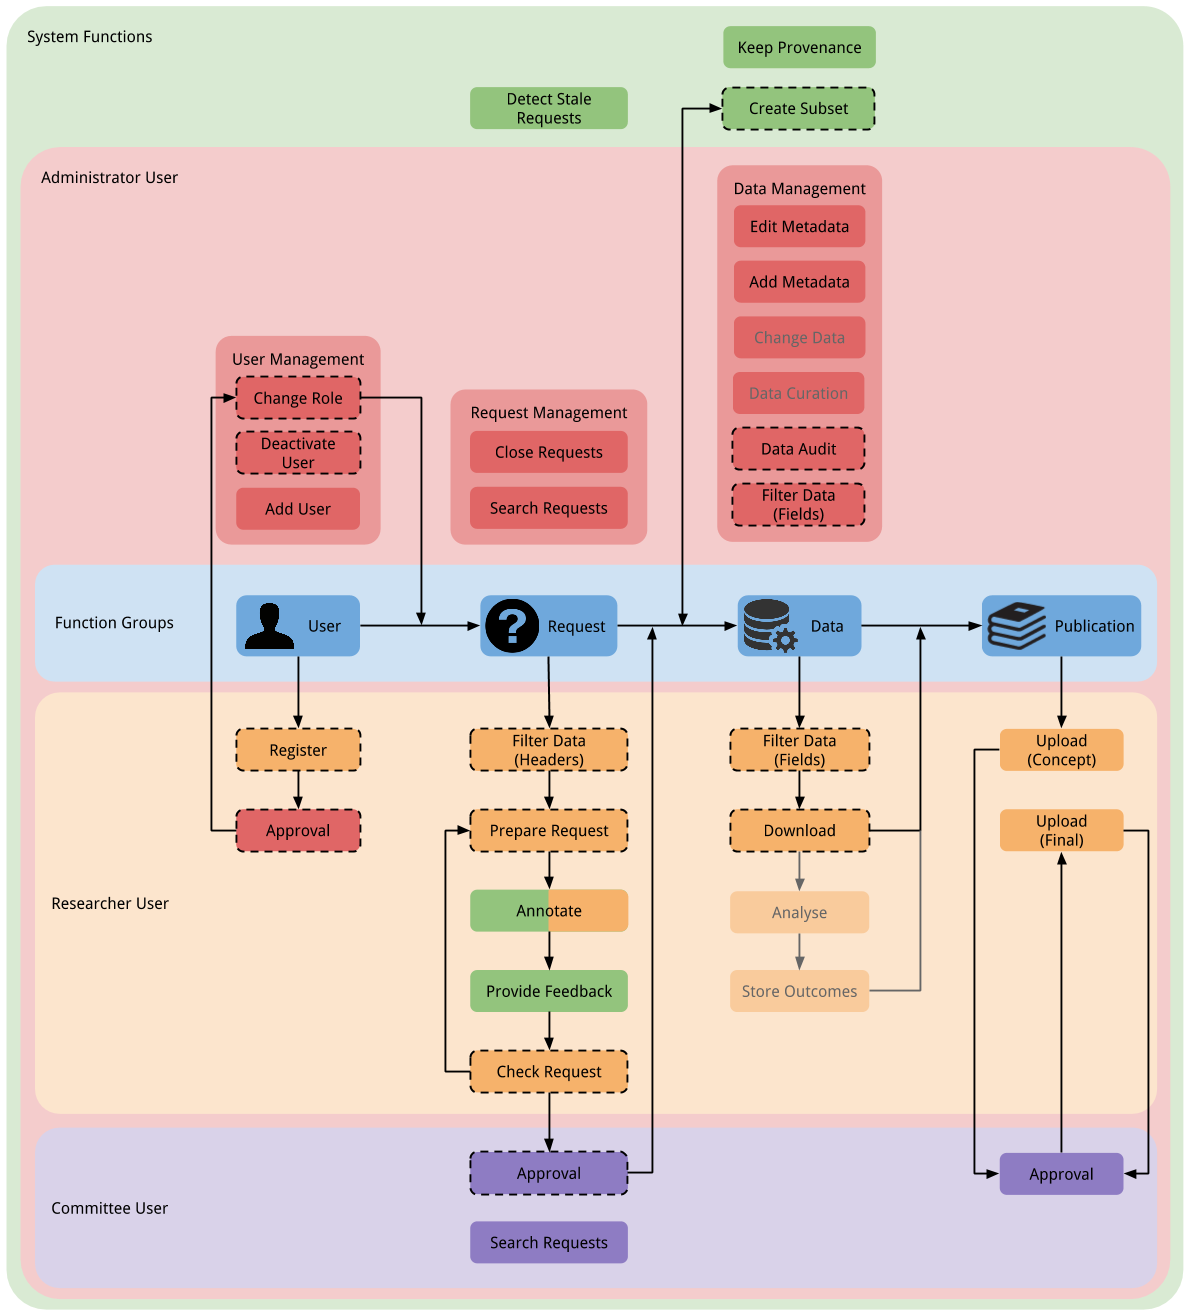
\includegraphics[width=1.0\linewidth]{images/functions-in-workflow}
	\caption{
		Gateway functions according to function groups, actors, and usage within the research workflow.
		Vertical columns represent different function groups, colours are used for different user roles, and arrows indicate sequence of actions.
		Greyed-out functions are deemed less important, which was an outcome of the brainstorm session (see section \ref{brainstorm}).
	}
	\label{fig:functions-workflow}
\end{figure}